\documentclass[10pt,conference,letterpaper]{IEEEtran}

\IEEEoverridecommandlockouts
% The preceding line is only needed to identify funding in the first footnote. If that is unneeded, please comment it out.
%Template version as of 6/27/2024

\usepackage{cite}
\usepackage{amsmath,amssymb,amsfonts}
\usepackage{optidef}
\usepackage{algorithm}
\usepackage{algorithmic}
\usepackage{graphicx}
\usepackage{textcomp}
\usepackage{xcolor}
\usepackage{booktabs}
\usepackage{multirow}
% \usepackage{microtype}
\def\BibTeX{{\rm B\kern-.05em{\sc i\kern-.025em b}\kern-.08em
    T\kern-.1667em\lower.7ex\hbox{E}\kern-.125emX}}

% \usepackage[style=ieee]{biblatex}
% \addbibresource{reference.bib}
\usepackage[colorlinks=true, linkcolor=blue, citecolor=blue, urlcolor=blue]{hyperref}

\begin{document}

\title{ADAPT-GUAV: Training-Inference Separation for Trajectory Generalization Design in Dynamic Data Collection Networks}

\author{
    \IEEEauthorblockN{Pengfei Wu,\IEEEmembership{~Member, IEEE},~Fu Xiao,\IEEEmembership{~Member, IEEE},~Chao Sha,~Haiping Huang}

    \IEEEauthorblockA{
    Nanjing University of Posts and Telecommunications, Nanjing, China\\
    Email: \{wupf, xiaof,shac and hhp\}@njupt.edu}}
% \author{\IEEEauthorblockN{1\textsuperscript{st} Given Name Surname}
% \IEEEauthorblockA{\textit{dept. name of organization (of Aff.)} \\

% \textit{name of organization (of Aff.)}\\
% City, Country \\
% email address or ORCID}
% \and
% \IEEEauthorblockN{2\textsuperscript{nd} Given Name Surname}
% \IEEEauthorblockA{\textit{dept. name of organization (of Aff.)} \\
% \textit{name of organization (of Aff.)}\\
% City, Country \\
% email address or ORCID}
% \and
% \IEEEauthorblockN{3\textsuperscript{rd} Given Name Surname}
% \IEEEauthorblockA{\textit{dept. name of organization (of Aff.)} \\
% \textit{name of organization (of Aff.)}\\
% City, Country \\
% email address or ORCID}
% \and
% \IEEEauthorblockN{4\textsuperscript{th} Given Name Surname}
% \IEEEauthorblockA{\textit{dept. name of organization (of Aff.)} \\
% \textit{name of organization (of Aff.)}\\
% City, Country \\
% email address or ORCID}
% \and
% \IEEEauthorblockN{5\textsuperscript{th} Given Name Surname}
% \IEEEauthorblockA{\textit{dept. name of organization (of Aff.)} \\
% \textit{name of organization (of Aff.)}\\
% City, Country \\
% email address or ORCID}
% \and
% \IEEEauthorblockN{6\textsuperscript{th} Given Name Surname}
% \IEEEauthorblockA{\textit{dept. name of organization (of Aff.)} \\
% \textit{name of organization (of Aff.)}\\
% City, Country \\
% email address or ORCID}
% }

\maketitle

\begin{abstract}
Efficient trajectory planning for Unmanned Aerial Vehicles in Internet of Things applications presents significant challenges when network topologies change dynamically. Traditional approaches often require extensive redesign or retraining, limiting their practical application in resource-constrained environments. This paper presents a training-inference separation framework that addresses these limitations through three interconnected components. We introduce a Complexity Assessment that evaluates the computational difficulty of trajectory optimization problems based on network topology characteristics. We develop a topology-driven instance generator capable of producing IoT device configurations across various spatial patterns, from uniformly distributed to highly clustered arrangements, enabling progressive learning paradigms. We implement an execution strategy where models trained offline can efficiently generate near-optimal UAV trajectory when confronted with previously unseen IoT network configurations. Evaluation results demonstrate our framework's dual advantages of effective cross-scenario adaptability across varied node distributions without environment-specific redesigns and efficient within-scenario generalization when interest nodes are dynamically added or removed. Experiments show 98.2\% optimality while reducing computation time by up to 99.7\% compared to exact solvers, making this approach suitable for resource-constrained UAVs operating in dynamic IoT environments.
\end{abstract}

\begin{IEEEkeywords}
Unmanned Aerial Vehicles, Internet of Things, trajectory generalization, dynamic networks, machine learning, training-inference separation
\end{IEEEkeywords}


\section{Introduction}
\label{sec:introduction}
% Background, importance, and challenges of UAV trajectory planning in IoT networks
% Brief overview of the problem and existing approaches
% Introduce TGP and its significance
% Highlight the limitations of existing approaches
% Briefly introduce ADAPT-GUAV and its advantages
% Outline the contributions of the paper
% Organization of the remaining sections

The Internet of Things (IoT) has revolutionized numerous industries by enabling ubiquitous sensing, computing and control through interconnected smart devices. As IoT networks continue to expand in scale and diversity, efficient data collection becomes increasingly challenging, particularly in large-scale deployments with spatially distributed nodes. Unmanned Aerial Vehicles (UAVs) have emerged as a promising solution for providing on-demand service to IoT devices due to their mobility, flexibility, and ability to operate in diverse environments \cite{DBLP:journals/jsac/ZhaoLHHPNQ25,journals/tsc/RoyTY25,DBLP:journals/tmc/GaoZ24}. However, designing optimal UAV trajectory remains a complex challenge that requires balancing multiple constraints including energy consumption, service quality, and adaptability to environmental variations.




UAV trajectory planning in IoT networks has attracted significant research attention in recent years. Traditional approaches typically formulate this as an optimization problem, aiming to minimize energy consumption or maximize service coverage while adhering to UAV mobility constraints \cite{DBLP:journals/tcom/ZhuZLLY24, DBLP:journals/comcom/FathollahiFA24}. These methods often use mathematical programming, heuristic algorithms, or reinforcement learning to compute optimal flight trajectory \cite{DBLP:journals/tiv/AdilSMAFJ24}. Although these approaches can achieve satisfactory performance in specific scenarios, they suffer from limited generalizability across diverse deployment environments and incur substantial computational overhead when adapting to dynamic network conditions.


UAV-assisted IoT networks operate across diverse deployment scenarios, each presenting unique spatial characteristics that significantly influence trajectory optimization. In environmental monitoring applications, sensors are sparsely distributed across large geographical areas, requiring extensive flight trajectory that balance coverage and energy efficiency \cite{DBLP:journals/iotj/LiuZ22a}. Urban deployments, conversely, feature high-density device clusters with non-uniform distributions and physical obstacles that constrain UAV movements \cite{DBLP:journals/tip/DaiZFQZY24}. Agricultural monitoring systems typically follow structured grid patterns with seasonal variations in data collection requirements, while industrial environments present precisely arranged devices with strict service timing requirements along production lines. These spatial distribution patterns fundamentally determine the efficiency of data collection strategies \cite{DBLP:journals/eswa/LiuLYZWS23,DBLP:journals/iotj/LiWSZCJ24}. 

Further complicating this challenge is the dynamic nature of IoT networks, where devices continuously join the network through new deployments or reactivations, while others leave due to energy depletion, maintenance requirements, or environmental factors \cite{DBLP:journals/tmc/ChenQSW25}. This spatial-temporal variability creates an evolving operational environment where trajectory solutions optimized for one configuration quickly become suboptimal as the network topology changes. The substantial diversity and dynamic characteristics of these deployment scenarios highlight the need for trajectory planning approaches that can effectively generalize across different spatial distributions and adapt to network changes without requiring complete recalculation.



To address these challenges, we formulate the Trajectory Generalization Problem (TGP), which focuses on developing UAV trajectory planning algorithms capable of generalizing across diverse deployment scenarios and adapting to dynamic network changes. TGP represents a fundamental shift from conventional trajectory optimization approaches that typically compute optimal trajectory for specific static configurations. The core insight underlying TGP is that despite the considerable variation in IoT deployment configurations, these deployments often exhibit common structural patterns and characteristics that can be systematically learned and exploited for efficient trajectory planning. By capturing these intrinsic patterns, a generalized trajectory planning framework can rapidly generate near-optimal flight paths for previously unseen device distributions without requiring complete recomputation.


Existing approaches fall short in addressing TGP due to several limitations. First, optimization-based methods require complete environment information and incur high computational overhead, making them impractical for real-time applications in dynamic networks. Second, reinforcement learning approaches typically train agents for specific environments, limiting their generalizability to unseen scenarios. Third, most existing works overlook the dynamic nature of IoT networks, assuming static node distributions throughout the UAV service period.

In this paper, we propose ADAPT-GUAV (ADaptive And Practical Trajectory planning with Generalization for UAVs), a novel framework that addresses TGP through a training-inference separation approach. ADAPT-GUAV leverages Curriculum Learning techniques to extract generalizable patterns from diverse deployment scenarios during an offline training phase. This knowledge is then utilized to enable rapid online trajectory planning that can adapt to both environment variations and dynamic node changes, without requiring expensive recomputation of optimal paths. Our approach achieves a balance between trajectory optimality, computational efficiency, and adaptability that is crucial for practical UAV deployments in IoT networks.





The contributions of this paper are as follows:

\begin{itemize}
    \item We formulate the Trajectory Generalization Problem for UAV-assisted IoT networks and identify the limitations of existing approaches in addressing this problem.
    \item We propose ADAPT-GUAV, a training-inference separation framework that enables efficient and adaptive trajectory planning across diverse IoT deployment scenarios.
    \item We design a novel neural network architecture that captures the spatial characteristics of IoT deployments and translates them into optimal UAV trajectory.
    \item We develop an online adaptation mechanism that allows UAVs to quickly adjust their trajectory in response to dynamic node changes.
    \item We conduct comprehensive experiments on both synthetic and real-world datasets, demonstrating that ADAPT-GUAV outperforms state-of-the-art methods in terms of energy efficiency, service quality, and computational overhead.

\end{itemize}


% The remainder of this paper is organized as follows. Section II reviews related work on UAV trajectory planning. Section III presents the system model and problem formulation. Section IV describes the ADAPT-GUAV framework in detail. Section V presents the experimental results and performance evaluation. Finally, Section VI concludes the paper and discusses future research directions.


\section{Related Work} 
\label{sec:related_work}

In this section, we review existing literature related to UAV trajectory planning in IoT networks and Machine Learning (ML)-based solutions for dynamic IoT environments.

\subsection{UAV Trajectory Planning in IoT Networks}


UAV trajectory planning for IoT service applications has been extensively studied using various approaches. Existing works can be broadly categorized into optimization-based and learning-based approaches.

\subsubsection{Optimization-Based Approaches}
Traditional optimization based trajectory planning formulates the problem as mathematical optimization with predefined objectives and constraints. Zeng et al. \cite{DBLP:journals/twc/ZengXZ19} proposed an energy-efficient UAV trajectory optimization framework that minimizes propulsion energy consumption while satisfying communication requirements. Zhao et al. \cite{DBLP:journals/jsac/ZhaoLHHPNQ25} formulated a joint optimization problem for content caching, service placement, and task offloading in UAV-enabled mobile edge computing networks to maximize quality-of-experience while meeting resource constraints. Liu et al. \cite{DBLP:journals/tvt/LiuLCH19} developed a multi-UAV cooperative trajectory optimization method based on genetic algorithms to maximize network coverage in IoT scenarios. For specific deployment environments, specialized optimization techniques have been proposed. Hu et al. \cite{DBLP:journals/iotj/HuWCCC22} developed a joint altitude and resource allocation algorithm using successive convex approximation for UAV-enabled urban emergency communications to maximize uplink throughput. For agricultural applications, Liu et al. \cite{DBLP:journals/eswa/LiuLYZWS23} proposed a multi-mechanism improved grey wolf optimization algorithm to enhance UAV trajectory planning efficiency across various field scales. However, these optimization approaches are typically tailored to specific deployment scenarios and require complete information about IoT device distributions, making them less adaptable to diverse environments and dynamic network changes.




\subsubsection{Learning-Based Approaches}

Machine learning techniques have recently been applied to UAV trajectory planning to address limitations of optimization-based methods. Reinforcement learning (RL) has emerged as a promising approach due to its ability to learn optimal policies through environment interaction. Wang et al. \cite{DBLP:journals/tmc/WangWPA23} employed deep reinforcement learning for jointly optimizing UAV trajectory and passive beamforming in intelligent reflecting surface-aided communications. Similarly, Song et al. \cite{DBLP:journals/tmc/SongDXLYX24} proposed a multi-objective reinforcement learning approach for energy-efficient trajectory optimization with wireless charging in UAV-assisted mobile edge computing. Furthermore, Huang et al. \cite{DBLP:journals/tmc/HuangWWYFSWL25} developed a learning-based approach for timely monitoring of points-of-interest with UAVs, while Zhu et al. \cite{DBLP:journals/tmc/ZhuCWHLY24} introduced collaborative reinforcement learning for 3D UAV tracking trajectory design. More recently, Zhou et al. \cite{DBLP:journals/tmc/ZhouXZYW24} developed a symmetry-augmented multi-agent reinforcement learning framework for scalable UAV trajectory design and user scheduling that enhances network performance through structural symmetry exploitation. Ning et al. \cite{DBLP:journals/tmc/NingYWSGJ24} proposed a multi-agent deep reinforcement learning approach for UAV trajectory optimization that effectively handles differentiated service requirements across diverse user groups. Despite these advances, existing learning-based approaches face challenges in generalizing across diverse IoT deployment environments, as they are typically trained and tested on similar scenarios.


\subsection{ML-Based Solutions for Dynamic IoT Networks}

The dynamic nature of IoT networks, characterized by devices joining and leaving the network, poses significant challenges for UAV trajectory planning.

\subsubsection{Transfer Learning and Federated Learning}
Transfer learning and domain adaptation techniques have been explored to enhance the adaptability of UAV control systems to changing environments. Liu et al. \cite{DBLP:conf/mobicom/0001M0HJ024} introduced a UAV-assisted integrated sensing and communication framework for emergency rescue activities, which employs transfer deep reinforcement learning to enable UAVs to adapt their navigation and communication policies across different urban scenarios. Similarly, Karmakar et al. \cite{DBLP:journals/tmc/KarmakarKA24a} proposed a federated learning-based approach for optimizing UAV trajectory control and power management, allowing UAVs to collaboratively learn and adapt to diverse mobile edge computing service environments.

Specifically addressing IoT networks, Ji et al. \cite{DBLP:journals/tmc/JiZC23} proposed a decoupled user association and trajectory design framework using multi-agent deep reinforcement learning, enabling UAVs to adaptively serve dynamic IoT devices in full-duplex multi-UAV networks. Additionally, Cui et al. \cite{DBLP:journals/tmc/CuiYWFH24} introduced a data value-based asynchronous federated learning approach for UAV swarms, allowing them to collaboratively adapt to unstable communication scenarios often encountered in IoT deployments. However, these approaches typically require substantial online computation for adaptation, limiting their applicability in resource-constrained UAV platforms.

\subsubsection{Training-Inference Separation}

Training-inference separation has emerged as a paradigm for deploying machine learning models in resource-constrained environments. This approach conducts computationally intensive training offline and enables lightweight inference on edge devices. Shao et al. \cite{DBLP:journals/tmc/ShaoYXSCX24} developed a deep reinforcement learning-based resource management framework for UAV-assisted mobile edge computing, which performs the complex optimization offline to ensure robust performance against jamming attacks in resource-constrained UAV platforms. Similarly, Ren et al. \cite{DBLP:journals/tmc/RenLMLWZLD24} introduced an intelligent adaptive gossip-based broadcast protocol for UAV-MEC systems, leveraging multi-agent deep reinforcement learning for the computationally intensive coordination while enabling efficient on-device execution. Training-inference separation approaches have shown promise in enhancing the practicality of deploying advanced machine learning on resource-constrained UAV platforms. However, these methods often rely on accurate environment models during offline training, limiting their ability to generalize to unforeseen deployment scenarios.


For IoT networks specifically, Ji et al. \cite{DBLP:journals/tmc/JiZC23} developed a joint trajectory and communication design framework for cache-enabled UAVs in cellular networks, which employs deep reinforcement learning to adaptively serve dynamic IoT device distributions. Additionally, Dai et al. \cite{DBLP:journals/tmc/DaiLHWLT23} proposed a delay-sensitive energy-efficient UAV crowdsensing approach using deep reinforcement learning, enabling rapid adaptation to varying IoT device densities and mobility patterns. However, existing works predominantly focus on single-environment scenarios and lack the ability to generalize across diverse IoT deployment patterns.



% The reviewed literature reveals a significant research gap in UAV trajectory planning for IoT networks: existing approaches either lack generalization capability across diverse IoT deployment environments or require substantial online computation for adaptation to dynamic network changes. Our proposed ADAPT-GUAV framework addresses these limitations by leveraging a training-inference separation approach that enables efficient generalization across diverse environments while maintaining adaptability to dynamic changes.



\section{System Model}
\begin{figure}[!t]
    \centering
    \includegraphics[width=0.45\textwidth]{fig/HAG系统模型.png}
    \caption{Illustration of the adaptability and generalization of UAV-enabled IoT networks across Diverse environments.}
    \label{fig:trajectory_generalization}
\end{figure} 

% As illustrated in Fig.~\ref{fig:trajectory_generalization}, 


In this section, we present the system model for the UAV-assisted IoT data collection scenario and formally define the Trajectory Generalization Problem (TGP). We begin by describing the network architecture, followed by the UAV mobility and energy consumption model, IoT device distribution model. Finally, we define the performance metrics used to evaluate our proposed approach.

\subsection{Network Model}

We consider a UAV-assisted IoT data collection system consisting of a Base Station (BS), a set of UAVs $\mathcal{U} = \{1,2,...,U\}$ serving a set of IoT devices $\mathcal{D} = \{1,2,...,D\}$ distributed across a geographical area $\mathcal{A} \subset \mathbb{R}^2$. The base station is assumed to be located at a fixed 3D position $\mathbf{q}_{BS} = [x_{BS}, y_{BS}, z_{BS}]^T$. Each UAV $u \in \mathcal{U}$ operates at a fixed altitude $h_u$, with a maximum flight time $T$ determined by its battery capacity. The position of UAV $u$ at time $t$ is denoted by $\mathbf{q}_u(t) = [x_u(t), y_u(t), h_u]^T$, where $[x_u(t), y_u(t)]^T \in \mathcal{A}$ represents the horizontal coordinates. Each IoT device $d \in \mathcal{D}$ is characterized by its position $\mathbf{w}_d = [x_d, y_d, 0]^T$, data size $B_d$. The devices are assumed to be static during a UAV mission, but their existence in the network may be dynamic, with devices joining or leaving the network over time.

To address the potential inefficiencies or unreliability of direct ground-to-base-station communication from IoT devices, we employ UAVs to facilitate data collection and relaying. Each IoT device $d$ initially attempts to transmit data to the base station via Wi-Fi HaLow (IEEE 802.11ah). However, when direct communication is limited, UAVs $\mathcal{U}$ are deployed to establish temporary, high-quality communication links with the IoT devices. By strategically positioning each UAV $u$ at a fixed altitude $h_u$ with adjustable horizontal coordinates $[x_u(t), y_u(t)]^T$, we optimize the elevation angle $\theta_{u,d}(t) = \sin^{-1}(h_u/\|\mathbf{q}_u(t) - \mathbf{w}_d\|)$ and the distance $d_{u,d}(t) = \|\mathbf{q}_u(t) - \mathbf{w}_d\|$ to the IoT device $d$. This strategic positioning aims to maximize the probability of a strong Line-of-Sight (LoS) path and minimize the impact of obstructions, thereby enhancing the data transmission rate from the IoT devices towards the base station via the UAV.




%For the communication model, both UAV-ground and ground-to-ground communications are typically modeled using a probabilistic Air-to-Ground channel, incorporating LoS and NLoS conditions. To simplify the analysis, we propose leveraging the UAV’s mobility to position it at a fixed altitude with adjustable horizontal coordinates. This allows us to optimize the elevation angle and distance to the target IoT device, thereby maximizing the probability of establishing a strong LoS path and minimizing the impact of obstructions.



Under this simplified approach, we consider only the LoS component of the Air-to-Ground channel. The expected channel gain between UAV $u$ and device $d$ is approximated by:

\begin{equation}
h_{u,d}^{\text{LoS}}(t) = \sqrt{\beta_0 d_{u,d}^{-\alpha}(t)K/(K+1)},
\end{equation}

where $d_{u,d}(t) = \|\mathbf{q}_u(t) - \mathbf{w}_d\|$ is the distance between the UAV and the device, $\beta_0$ is the reference channel gain at a unit distance, $\alpha$ is the path loss exponent, and $K$ is the Rician K-factor. %The elevation angle $\theta_{u,d}(t)$ still plays a role in determining the likelihood of maintaining a strong LoS link through strategic positioning.

The achievable data rate $R_{u,d}(t)$ between UAV $u$ and device $d$ at time $t$ under this simplified LoS channel model is:
\begin{equation}
R_{u,d}(t) = B\log_2\left(1 + \frac{P_{comm}(t) |h_{u,d}^{\text{LoS}}(t)|^2}{\sigma^2 + \sum_{i\in\{\mathcal{U}\setminus u\}} P_i(t) |h_{i,d}^{\text{LoS}}(t)|^2}\right),
\end{equation}
where $B$ is the system bandwidth, $P_{comm}(t)$ is the transmit power of UAV $u$, and $\sigma^2$ is the noise power. 

%Therefore, the optimization of the UAV's trajectory is fundamentally aimed at enhancing the data rate from the IoT devices to the base station by ensuring favorable LoS conditions through strategic positioning, which in turn maximizes $R_{u,d}(t)$. We continue to assume a reliable, high-capacity link for data offloading from the UAV to the base station.


% The mobility of each UAV $u \in \mathcal{U}$ is subject to kinematic constraints that govern its movement capabilities. The horizontal velocity $\mathbf{v}_u(t) = [\dot{x}_u(t), \dot{y}_u(t)]^T$ must satisfy $||\mathbf{v}_u(t)|| \leq V_{max}$, where $V_{max}$ represents the maximum achievable speed of the UAV platform. Similarly, the acceleration $\mathbf{a}_u(t) = [\ddot{x}_u(t), \ddot{y}_u(t)]^T$ is bounded by $||\mathbf{a}_u(t)|| \leq A_{max}$, with $A_{max}$ denoting the maximum allowable acceleration determined by the UAV's physical limitations. These constraints ensure realistic motion profiles that account for the inertia and mechanical capabilities of typical rotary-wing UAVs.


\subsection{UAV Mobility and Energy Consumption Model}
\label{subsec:mobility_energy_model}
% Assuming this is part of a subsection, e.g., within \subsection{UAV Mobility and Energy Consumption Model}

The mobility of each Unmanned Aerial Vehicle (UAV) $u$ throughout the mission duration $T$ is governed by kinematic constraints. These constraints apply to its trajectory $q_u(t)$, its horizontal velocity $\mathbf{v}_u(t) = [\dot{x}_u(t), \dot{y}_u(t)]^T$, and its horizontal acceleration $\mathbf{a}_u(t) = [\ddot{x}_u(t), \ddot{y}_u(t)]^T$. As detailed in Equations~\eqref{eq:constraints_10a} and \eqref{eq:constraints_10b}, these ensure that each UAV starts from and returns to its depot, remains within the designated operational area $\mathcal{A}$, and adheres to limits on maximum velocity $V_{\text{max}}$ and acceleration $A_{\text{max}}$.


\begin{align}
    & q_u(0)=q_u(T)=\mathbf{q}_{BS}, \quad &&[x_u(t),y_u(t)]^T \in \mathcal{A}  \label{eq:constraints_10a} \\
    & ||\mathbf{v}_u(t)|| \leq V_{\text{max}}, \quad &&||\mathbf{a}_u(t)|| \leq A_{\text{max}} \label{eq:constraints_10b}
\end{align}




The total energy expenditure $E_u$ of UAV $u$ over the mission must not exceed its battery capacity $E_{\text{max}}$, formulated as:
\begin{equation}
E_u = \int_{0}^{T} P_{u}(t) \, dt \leq E_{\text{max}}.
\label{eq:total_energy_expenditure}
\end{equation}
The instantaneous total power consumption $P_{u}(t)$ is primarily determined by the UAV's flight dynamics and communication activities. It can be expressed as the sum of two main components, propulsion power $P_{\text{prop}}(\mathbf{v}_u(t))$ and communication power $P_{\text{comm}}(t)$:


\begin{equation}
P_{u}(t) = P_{\text{prop}}(\mathbf{v}_u(t)) + P_{\text{comm}}(t).
\label{eq:instantaneous_power_consumption}
\end{equation}

The propulsion power, $P_{\text{prop}}(\mathbf{v}_u(t))$, is a function of the UAV's instantaneous velocity $\mathbf{v}_u(t)$. We adopt a standard aerodynamic model for rotary-wing UAVs based on fundamental flight dynamics principles, as established in the reference work by Zeng et al. ~\cite{DBLP:journals/twc/ZengXZ19}. %This model, which has become widely accepted in the field, particularly captures the key characteristics of UAV forward flight. 
This comprehensive propulsion model inherently accounts for the power required for all flight states, including hovering (i.e., when $\|\mathbf{v}_u(t)\| \approx 0$, the model yields the necessary hovering power), as well as flight at various speeds and accelerations.





The communication power, $P_{\text{comm}}(t)$, represents the power consumed by the onboard wireless transceivers for data transmission to other UAVs or the base station, and for receiving data or command signals. This component typically depends on the transmission power level, data rate, and communication hardware specifics.


% This formulation ensures that the power consumption accurately reflects the UAV's state (e.g., its speed and communication load) without double-counting power components like hovering, as the propulsion model $P_{\text{prop}}(\mathbf{v}_u(t))$ is comprehensive.

Collision constraints are not explicitly modeled in our trajectory optimization, as these are assumed to be handled by dedicated, high-rate onboard controllers using local sensing, allowing our focus to remain on energy-efficient trajectory design compatible with standard UAV autonomy systems.

\subsection{IoT Device Distribution Model}
\label{subsec:iot_distribution}

To model the spatial distribution of IoT devices across diverse deployment scenarios, we employ a unified parametric approach. The device density function $\mathcal{D}(x,y)$ is defined as a mixture of a spatially random component, modeled by a Poisson process $\mathcal{P}_\lambda(x,y)$, and a spatially clustered component, represented by a weighted sum of multivariate Gaussian distributions $\mathcal{N}(\mathbf{\mu}_c, \mathbf{\Sigma}_c)$:
\begin{equation}
\mathcal{D}(x,y) = (1-\alpha) \cdot \mathcal{P}_\lambda(x,y) + \alpha \cdot \sum_{c=1}^C w_c \cdot \mathcal{N}(\mathbf{\mu}_c, \mathbf{\Sigma}_c).
\end{equation}
The clustering intensity is controlled by the parameter $\alpha \in [0,1]$. By adjusting $\alpha$ and the parameters of the Gaussian components (weights $w_c$, centroids $\mathbf{\mu}_c$, and covariance matrices $\mathbf{\Sigma}_c$), the model can effectively represent various deployment characteristics, as illustrated by the following representative scenarios:

\begin{enumerate}
    \item \textbf{Sparse Random Distribution (Forest)}: A purely random deployment is achieved by setting $\alpha = 0$, resulting in $\mathcal{D}_{1}(x,y) = \mathcal{P}_\lambda(x,y)$, where a low intensity $\lambda \leq 0.1$ indicates a sparse distribution.

    \item \textbf{Dense Clustered Distribution (Urban)}: Urban environments, characterized by dense clusters of devices, are modeled with a high clustering intensity (e.g., $\alpha \rightarrow 0.8$). With equal cluster weights $w_c = 1/C$ and isotropic covariance matrices $\mathbf{\Sigma}_c = \sigma^2\mathbf{I}$, the density becomes $\mathcal{D}_{2}(x,y) = 0.2\mathcal{P}_\lambda(x,y) + 0.8\sum_{c=1}^{C} \frac{1}{C}\mathcal{N}(\mathbf{\mu}_c, \sigma^2\mathbf{I})$, where $C$ is the number of clusters and $\sigma$ controls their spread.

    \item \textbf{Grid-Based Distribution (Agriculture)}: Agricultural deployments often exhibit a grid-like structure. This can be modeled by considering a dominant clustering component ($\alpha \rightarrow 1$) with highly localized clusters, approximated by Dirac delta functions $\delta(x-x_i,y-y_j)$ located at the grid points $(x_i, y_j)$ with uniform weights $1/(mn)$, yielding $\mathcal{D}_{3}(x,y) = \sum_{i=1}^m\sum_{j=1}^n \frac{1}{mn}\delta(x-x_i,y-y_j)$.

    \item \textbf{Structured Linear Distribution (Factory)}: Linear or corridor-like deployments, common in factory settings, are modeled with $\alpha = 1$, anisotropic covariance matrices $\mathbf{\Sigma}_c = \text{diag}(\sigma_x^2, \sigma_y^2)$ oriented along the linear structures, and cluster weights $w_c = c^{-2.5}/Z$ to introduce structure. The resulting density is $\mathcal{D}_{4}(x,y) = \sum_{c=1}^L \frac{c^{-2.5}}{Z}\mathcal{N}\left(\mathbf{\mu}_c, \begin{bmatrix} \sigma_x^2 & 0 \\ 0 & \sigma_y^2 \end{bmatrix}\right)$, where $Z$ is a normalization constant and $\mathbf{\mu}_c$ are centroids aligned along the linear structures.

\end{enumerate}

This unified model, through its parametric flexibility, enables the representation of a wide spectrum of IoT deployment topologies relevant to various application scenarios.


% These quantitative measures, IoT device coverage $\mathcal{C}$, average system througput $\mathcal{T}$, and system energy efficiency $\mathcal{E}_{sys}$, provide a framework for evaluating the UAV-assisted data collection service.





\subsection{Service Model}
\label{subsec:service_model}

The primary service provided by the UAVs is data collection from the distributed IoT devices. Each IoT device $d \in \mathcal{D}$ requires $B_d$ bits of data to be successfully uploaded to a visiting UAV within the mission duration $T$. Due to potential interference and varying channel conditions, a device $d$ can associate with at most one UAV $u$ at any given time $t$. We introduce a binary association variable $a_{u,d}(t) \in \{0, 1\}$, where $a_{u,d}(t)=1$ if and only if UAV $u$ is scheduled to collect data from device $d$ at time $t$. This leads to the constraint:
\begin{equation}
\label{eq:association_constraint}
\sum_{u \in \mathcal{U}} a_{u,d}(t) \leq 1, \quad \forall d \in \mathcal{D}, \forall t \in [0, T].
\end{equation}

% To guarantee complete device coverage, we require that each device receives sufficient connection time:
% \begin{equation}
% \label{eq:coverage_constraint}
% \int_{0}^{T} \sum_{u \in \mathcal{U}} a_{u,d}(t) dt \geq \tau_d, \quad \forall d \in \mathcal{D}
% \end{equation}
% where $\tau_d$ is the minimum required connection time for device $d$. 
The total data collected from device $d$ by all UAVs throughout the mission duration $T$ is denoted $B_{d}^{\text{coll}}$, and is calculated as:
\begin{equation}
\label{eq:collected_data_definition}
B_{d}^{\text{coll}} = \sum_{u \in \mathcal{U}} \int_{0}^{T} a_{u,d}(t) R_{u,d}(t) dt.
\end{equation}

The service requirement for device $d$ is to collect a total of $B_d$ data. This requirement is formally expressed as the following constraint:
\begin{equation}
\label{eq:service_requirement_condition}
B_{d}^{\text{coll}} \geq B_d.
\end{equation}



\subsection{Performance Metrics}
\label{subsec:performance_metrics}
% Proposed Order: 1. Latency, 2. Integrity, 3. Throughput, 4. Energy
In this work, we consider UAV-assisted data collection as one instance of the broader spectrum of services that UAVs can provide to IoT devices. Other potential services include computation offloading, content caching, and search-and-rescue \cite{DBLP:conf/infocom/Sun0HM0024,DBLP:journals/jsac/ZhengZJ24,DBLP:journals/tmc/SoorkiAABCS25}. Our service model for UAV-assisted data collection focuses on the efficient and effective acquisition of data from IoT devices using UAVs.


To evaluate the performance of the UAV-assisted data collection service, we consider the following key performance indicators:

% \subsubsection{IoT Device Coverage (\texorpdfstring{$\mathcal{C}$}{C})}

% To evaluate the overall IoT device coverage throughout the entire mission duration $T$, we define the average coverage $\mathcal{C}$ as the time average of the instantaneous coverage $\mathcal{C}(t)$:
% \begin{equation} 
% \begin{split}
% \mathcal{C} &= \frac{1}{T} \int_{0}^{T} \mathcal{C}(t) \, dt \\
%             &= \frac{1}{T} \int_{0}^{T} \left( \frac{1}{|\mathcal{D}|} \sum_{d \in \mathcal{D}} \mathbb{I}\left( \sum_{u \in \mathcal{U}} a_{u,d}(t) \geq 1 \right) \right) \, dt.
% \end{split}
% \end{equation}
% The instantaneous coverage $\mathcal{C}(t)$ represents the fraction of devices covered at a specific time $t$. By integrating $\mathcal{C}(t)$ over the entire mission duration $T$ and dividing by $T$, the average coverage $\mathcal{C}$ provides a holistic measure of how well the IoT devices are served throughout the operation. A higher value of $\mathcal{C}$ indicates a better overall coverage performance of the UAV system. The objective related to coverage is typically to maximize this average coverage $\mathcal{C}$.

\subsubsection{Data Collection Latency ($\mathcal{L}$)}
Data collection latency $L_d$ for an IoT device $d$ is its waiting time, $L_d = t_{d,\text{start}} - t_{d,\text{ready}}$, representing the period from data readiness ($t_{d,\text{ready}}$) until a UAV initiates service ($t_{d,\text{start}}$). Key system-level aggregations of this latency are maximum latency $\mathcal L_{\text{max}} = \max_{d \in \mathcal{D}} \{L_d\}$ and the average latency $\mathcal{L}$




\begin{equation}
\mathcal{L} = \frac{1}{|\mathcal{D}|} \sum_{d \in \mathcal{D}} L_d.
\label{eq:avg_latency_terse}
\end{equation}

\subsubsection{Data Collection Integrity $(\mathcal{C})$}
We define $\mathcal{C}$ to quantify the completeness of data collection across all IoT devices by mission completion:
\begin{equation}
\mathcal{C} = \frac{1}{|\mathcal{D}|} \sum_{d \in \mathcal{D}} \mathbb{I}\left( B_d^{\text{coll}} \geq B_d \right),
\label{eq:c_comp_definition}
\end{equation}
where $\mathbb{I}(\cdot)$ is the indicator function. The indicator $\mathbb{I}\left( B_d^{\text{coll}}\geq B_d \right)$ is equal to 1 if the total data collected from device $d$ meets or exceeds its requirement $B_d$, and 0 otherwise. A higher value of $\mathcal{C}$ signifies that a larger proportion of the targeted IoT devices have had their data fully collected within the operational timeframe $T$. This metric thus directly captures the objective of ensuring comprehensive data retrieval from as many nodes as possible during the mission.



\subsubsection{Average System Throughput $(\mathcal{T})$}

The average system throughput is defined as the time-averaged rate at which data from IoT devices is successfully delivered to the base station:
\begin{equation}
\mathcal{T}= \frac{1}{T}\int_0^T\sum_{u \in \mathcal{U}} \sum_{d \in \mathcal{D}} a_{u,d}(t) R_{u,d \rightarrow BS}(t),
\end{equation}
where $R_{u,d \rightarrow BS}(t)$ is the data rate from UAV $u$ to the BS for data from device $d$.

\subsubsection{UAV Energy Utilization Efficiency $(\mathcal{E})$}

The average ratio of total data collected by each UAV to its total energy consumption:
\begin{equation}
\mathcal{E} = \frac{1}{|\mathcal{U}|} \sum_{u \in \mathcal{U}} \frac{\int_{0}^{T} \sum_{d \in \mathcal{D}} a_{u,d}(t) R_{u,d}(t) \, dt}{\int_{0}^{T} P_{u}(t) \, dt}.
\end{equation}

% \subsubsection{Data Collection Latency ($L_d, \bar{L}, L_{\text{max}}$)}

% Data collection latency $L_d$ for an IoT device $d$ is defined as its waiting time from when data is ready, until a UAV initiates data collection at that device. This metric focuses on UAV responsiveness in attending to devices and excludes subsequent device-to-UAV data transmission time and any UAV-to-Base Station communication delays. The primary system-level latency metrics considered are the average latency
% \begin{equation}
%     \bar{L} = \frac{1}{|\mathcal{D}|} \sum_{d \in \mathcal{D}} L_d, 
% \end{equation}
% and the maximum latency experienced by any device, $L_{\text{max}} = \max_{d \in \mathcal{D}} \{L_d\}.$ Minimizing these latency values is important for ensuring prompt UAV service initiation to the IoT devices.

Collectively, these performance metrics provide quantitative insights into critical aspects such as service promptness, mission completion success, overall data transfer efficiency, and energy sustainability. 

\section{Problem Formulation}
\label{sec:problem_formulation}
The Trajectory Generalization Problem (TGP) addresses generalized trajectory design for UAVs in low-altitude Internet of Things applications. This scenario involves UAVs collecting data across diverse IoT deployment environments (such as forest fire monitoring, smart city surveillance, agricultural monitoring, and commercial district supervision) while simultaneously accommodating the dynamic addition or removal of interest IoT devices (e.g., monitoring targets or data collection points). The objective is to rapidly optimize UAV trajectory that maintain robust adaptability across varied environments while maximizing system utility in dynamic settings. The formal definition of the problem is presented below.

\subsection{Trajectory Generalization Problem (TGP)}


Let $\mathcal{S}$ be a set of representative deployment scenarios, where each scenario $s \in \mathcal{S}$ defines a specific configuration of IoT devices $\mathcal{D}^{(s)}$, their locations $w_{d,s}$, data requirements $B_{d,s}$, and data ready times $t_{d,ready}^{s}$. The system comprises a set of UAVs $\mathcal{U}$ with the following characteristics for each scenario $s\in\mathcal{S}$ and each UAV $u\in\mathcal{U}$. The UAV trajectory are defined by $q_u^{(s)}(t)=[x_u^{(s)}(t),y_u^{(s)}(t),h_u]^{T}$ for $t\in[0,T]$, where $h_u$ represents the fixed operational altitude of UAV $u$ for scenario $s$. These trajectory implicitly determine the velocities $\mathbf{v}_u^{(s)}(t)$ and accelerations $\mathbf{a}_u^{(s)}(t)$ of each UAV. The IoT-UAV association schedule is characterized by binary variables $a_{u,d}^{(s)}(t)\in\{0,1\}$.%, where $a_{u,d}^{(s)}(t)=1$ indicates that UAV $u$ is actively collecting data from device $d\in\mathcal{D}^{(s)}$ at time $t$ in scenario $s$, while $a_{u,d}^{(s)}(t)=0$ signifies no data collection is occurring.



The objective of TGP is to maximize the expected system utility over all scenarios. The system utility is a weighted combination of the performance metrics. Let $\mathcal{C}_{s}$, $\mathcal{L}_{s}$, $\mathcal{T}_{s}$, and $\mathcal{E}_{s}$ denote the performance metrics for scenario $s$, respectively. The TGP can be formally expressed as the following optimization problem:



\begin{equation}
\begin{aligned}
\text{(P1): } \max_{\{q_u^{(s)}(t),a_{u,d}^{(s)}(t)\}} &\mathbb{E}_s[\omega_1 \mathcal{C}_s - \omega_2 \mathcal{L}_s + \omega_3 \mathcal{T}_s + \omega_4 \mathcal{E}_s]\\
\text{s.t.} &\quad \text{~\eqref{eq:constraints_10a},~\eqref{eq:constraints_10b},~\eqref{eq:total_energy_expenditure},~\eqref{eq:association_constraint},~\eqref{eq:service_requirement_condition}}
\end{aligned}
\end{equation}

\subsection{Optimization of TGP using Reinforcement Learning}
\label{subsec:optimization_tgp_rl}

The Trajectory Generalization Problem (P1) encompasses multiple objectives, diverse scenario configurations, and dynamic elements. Consequently, deriving its direct optimal solution is often computationally intractable for practical deployment environments. To establish a more tractable solution methodology, our initial strategy involves simplifying the TGP. This reduction entails focusing on a single, static deployment scenario and optimizing the trajectory for an individual UAV. Accordingly, the expectation over scenarios $\mathbb{E}_s[\cdot]$ and the scenario-specific superscript $(s)$ are omitted from all pertinent variables.

Within this simplified analytical framework, the principal objective becomes ensuring comprehensive Data Collection Integrity ($\mathcal{C}$). This implies a fundamental mandate that the UAV must visit and successfully retrieve the requisite data volume $B_d$ from all designated IoT devices. Such a condition necessitates the satisfaction of Constraint~\eqref{eq:service_requirement_condition} for all devices, thereby targeting $\mathcal{C}=1$ for the specified device set.

Given this integrity mandate as a baseline, the optimization focus shifts towards augmenting the Path Efficiency of the UAV's tour. The aggregate flight path length, or the total mission duration $T_u$, exerts considerable influence upon several key performance indicators. Minimization of the path length directly curtails propulsion energy consumption, a predominant component of $P_u(t)$ (refer to Equation~\eqref{eq:instantaneous_power_consumption}), thereby enhancing UAV Energy Utilization Efficiency ($\mathcal{E}$). 

Moreover, an optimally sequenced and shorter trajectory can facilitate earlier service initiation times $t_{d,\text{start}}$ for devices, relative to their data readiness times $t_{d,\text{ready}}$, which potentially diminishes both average and maximum Data Collection Latency ($\mathcal{L}$). While System Throughput ($\mathcal{T}$) is not the primary optimization target at this stage, expeditious tour completion can subsequently afford more opportunities for data offloading to the Base Station.

The simplified problem, designated (P2), is subsequently reformulated by leveraging principles from reinforcement learning (RL) methodologies applied to TSP-like sequencing challenges. The objective is to derive an optimal policy for the UAV to ascertain the visitation sequence for all devices in $\mathcal{D}$, commencing from and reverting to a central depot, i.e., the Base Station $\mathbf{q}_{BS}$.
Let $\mathbf{X} = \{x_1, x_2, \dots, x_N\}$ represent the set of $N=|\mathcal{D}|+1$ distinct 2D coordinates, where $x_1$ denotes the depot, and $x_2, \dots, x_N$ correspond to the IoT device locations. A tour is a permutation $\pi = [\pi_1, \pi_2, \dots, \pi_N]$ of these $N$ locations, where the policy typically determines the sequence starting from a fixed depot $\pi_1 = x_1$. The cost, or length, of such a tour $L(\pi, \mathbf{X})$ is its total Euclidean distance:
\begin{equation}
\label{eq:P2_rl_tsp_cost_revised}
L(\pi, \mathbf{X}) = ||x_{\pi_N} - x_{\pi_1}||_2 + \sum_{i=1}^{N-1} ||x_{\pi_{i+1}} - x_{\pi_i}||_2.
\end{equation}
The RL agent endeavors to acquire a policy $p_{M_{\theta}}(\pi|\mathbf{X})$ that minimizes the expected cost. This objective is realized through the minimization of the loss function $\mathcal{L}_{\theta}(\mathbf{X})$, defined consistently with \cite{DBLP:conf/aaai/ZhangZW022}:
\begin{equation}
\label{eq:P2_rl_loss_revised}
\text{(P2): } \min_{M_{\theta}} \quad \mathcal{L}_{M_{\theta}}(\mathbf{X}) = \mathbb{E}_{p_{M_{\theta}}(\pi|\mathbf{X})}[L(\pi, \mathbf{X})].
\end{equation}
The training process uses standard reinforcement learning methods like REINFORCE to produce valid routing solutions. This approach naturally creates complete tours that visit every target device exactly once and return to the starting base station, forming a proper closed loop. The minimization of $L(\pi, \mathbf{X})$ must adhere to the UAV's operational constraints. Specifically:
\begin{itemize}
    \item The UAV's movement between nodes must satisfy the flight dynamics constraints in Equations~\eqref{eq:constraints_10a} and~\eqref{eq:constraints_10b}. The RL environment enforces these constraints through either action space restrictions or state transition rules.
    \item The total tour distance $L(\pi, \mathbf{X})$ cannot exceed the UAV's maximum flight range, as defined by the energy model in Equation~\eqref{eq:total_energy_expenditure}. This limits how long each tour can be.
\end{itemize}
% This RL-centric formulation (P2) for single-UAV path optimization within a static scenario establishes a robust foundation. The acquisition of a policy for generating efficient tours primarily addresses data integrity (via the construction of tours encompassing all requisite devices), and secondarily targets energy efficiency and latency through cost minimization. The derived policies or resultant pathing strategies can subsequently inform or be integrated within more sophisticated architectures designed to address the full spectrum of the TGP, including multi-UAV coordination, adaptation to dynamic network topologies, and generalization capabilities across heterogeneous operational environments.
The RL-based formulation (P2) provides a fundamental solution for single-UAV path planning in static scenarios. The learned policy first ensures complete data collection by visiting all target devices, while also optimizing for shorter trajectory to improve energy efficiency and reduce latency. These single-UAV solutions can then be extended to more complex systems handling multiple UAVs, dynamic networks, and diverse operational environments.  

\section{The ADAPT-GUAV Framework}
\label{sec:adapt_uav}
% Overview of the proposed framework

This section introduces the ADAPT-GUAV framework. ADAPT-GUAV is designed to address the complexities of the Trajectory Generalization Problem (TGP) by leveraging a strategic separation of concerns: intensive offline training to build a robust, generalizable trajectory generation model, followed by efficient online inference for rapid adaptation in diverse and dynamic operational environments.

\subsection{Training-Inference Separation}

A fundamental design choice in ADAPT-GUAV is the separation of the training and inference phases. This approach is crucial for achieving both high performance and practical deployability.

Offline Training Phase focuses on solving the simplified, yet foundational, problem (P2) using reinforcement learning. As described in Section~\ref{subsec:optimization_tgp_rl}, an RL agent, is trained to develop a policy $p_{M_{\theta}}(\pi|\mathbf{X})$ that generates energy-efficient tours for a single UAV in static scenarios. This training process is computationally intensive, involving extensive exploration and learning over a wide variety of simulated IoT device distributions (derived from Section~\ref{subsec:iot_distribution}). The outcome of this phase is a highly optimized and generalizable policy, $M_{\theta}$, capable of determining near-optimal visitation sequences for a given set of device locations.

Once the policy $M_{\theta}$ is trained, it can be deployed for online trajectory generation. In this phase, when presented with a specific scenario (either static at the start of a mission or a dynamically updated state), the framework uses the pre-trained policy to rapidly infer an efficient UAV trajectory. This inference step is computationally lightweight, allowing for quick decision-making and trajectory adjustments. For instance, given the current locations of IoT devices $\mathbf{X}$ in an operational area, ADAPT-GUAV applies $M_{\theta}$ to swiftly calculate $L(\pi, \mathbf{X})$, forming the basis of the UAV's flight path.

The key advantage of this separation is that the heavy computational lifting is performed offline, making the online deployment efficient and responsive. This allows ADAPT-GUAV to quickly generate or adapt trajectories without requiring extensive re-computation in the field.

\subsection{From Static Scenarios to Dynamic Environments}

While the RL agent is trained on the simplified problem (P2) which assumes a static set of devices, the strong generalization capabilities of the learned policy are pivotal for ADAPT-GUAV's effectiveness in the dynamic and diverse environments envisioned by the TGP.

\textbf{Basis of Generalization:} The RL agent, by being exposed to a multitude of device configurations during training (reflecting the diverse distributions in Section~\ref{subsec:iot_distribution}), learns underlying heuristics and patterns for efficient path planning rather than memorizing solutions to specific instances. It learns how to connect points efficiently in a 2D space under given constraints. This inherent ability to generalize is a known strength of modern Curriculum Reinforcement Learning architectures when trained appropriately on diverse datasets in \cite{DBLP:conf/aaai/ZhangZW022}.

\textbf{Adapting to Dynamic IoT Networks:} The dynamic nature of IoT networks, where devices may join or leave, is handled through the rapid inference capabilities of the trained policy. When the set of active IoT devices $\mathcal{D}$ changes, this new set of locations $\mathbf{X}'$ is fed into the pre-trained policy $M_{\theta}$. The policy then generates a new, optimized tour $L(\pi', \mathbf{X}')$ for this updated configuration almost instantaneously. This \textit{re-plannin} is not a \textit{re-training} process but rather a new inference pass. The framework's ability to generalize means it can produce high-quality trajectories for these previously unseen configurations, maintaining system utility.

\textbf{Handling Diverse Environments:} The TGP solution maintains strong performance across different environments through comprehensive training. As detailed in Section~\ref{subsec:iot_distribution}, we train policy $M_{\theta}$ on diverse synthetic data covering various device distributions. This enables the policy to handle different spatial patterns without requiring environment-specific adjustments. The approach successfully learns universal routing principles that work across all these cases.


% Therefore, ADAPT-GUAV extends the solution from the static, single-UAV problem (P2) to the broader, dynamic TGP by relying on the generalization power of the offline-trained RL policy and its fast online inference. This allows for continuous adaptation to evolving device landscapes and mission requirements, forming the cornerstone of the framework's practical utility in real-world UAV-assisted IoT networks. While (P2) focuses on path efficiency for a single UAV to ensure data integrity and improve energy/latency, the rapid and generalizable nature of its solution provides a strong foundation for addressing the multi-faceted objectives of (P1) in more complex, multi-UAV scenarios (which can be explored as extensions, e.g., by partitioning tasks among UAVs, each using a version of this generalized policy).
Therefore, the ADAPT-GUAV framework expands the single-drone solution from P2 to dynamic scenarios using a pre-trained RL policy with fast online execution. This approach automatically adjusts to changing device locations and mission needs, making it practical for real-world IoT networks. The original P2 solution ensures reliable data collection while optimizing energy use and response time for the individual UAV. Its efficient and adaptable policy can then support more complex multi-UAV trajectory design required in P1. For implementation, the system can divide tasks among multiple drones, each running the same general routing policy.




\section{Algorithms}
\label{sec:algorithms}

The ADAPT-GUAV framework utilizes a two-phase algorithmic methodology. The initial phase encompasses a computationally intensive offline training period to establish a generalizable trajectory generation policy, $M_{\theta}$, by addressing the simplified formulation (P2). This policy is subsequently employed in the second phase for expeditious online inference to determine UAV trajectories.

\subsection{Offline Policy Optimization via Hardness-Adaptive Curriculum Learning for P2}

The primary objective of the offline phase is to train the policy $M_{\theta}$ to generate efficient sequence $\pi$ that minimize the length $L(\pi, \mathbf{X})$. Building upon the Hardness-Adaptive Curriculum Learning framework proposed in  \cite{DBLP:conf/aaai/ZhangZW022}, we develop an enhanced training algorithm. Our approach extends the original method by incorporating domain-specific adaptations for UAV routing scenarios. This methodology involves:
\subsubsection{Hardness Assessment} 
A key component of the curriculum is the quantitative assessment of instance hardness.
While our conceptualization of hardness emphasizes an instance's topological propensity to challenge the extant policy $M_{\theta}$'s learned heuristics, for a concrete quantitative measure, we employ a metric consistent with the principles outlined by Zhang et al.~\cite{DBLP:conf/aaai/ZhangZW022}.
The hardness $\mathcal{H}(X, M_{\theta})$ of a TSP instance $X = \{x_1, \dots, x_N\}$ for the current policy $M_{\theta}$ is defined as:
\begin{equation}
\mathcal{H}(X, M_{\theta}) = \frac{\mathcal{L}_{M_{\theta}}(X) - \mathcal{L}_{M'_{\theta}}(X)}{\mathcal{L}_{M'_{\theta}}(X)},
\label{eq:hardness_metric}
\end{equation}
where $\mathcal{L}_{M_{\theta}}(X) = \mathbb{E}_{p_{M_{\theta}}(\pi|X)}[L(\pi, X)]$ is the expected cost achieved by the current policy $M_{\theta}$ on instance $X$. $M'_{\theta}$ is a surrogate model obtained by greedily improving the current policy $M_{\theta}$ on instance $X$. $\mathcal{L}_{M'_{\theta}}(X)$ is the expected cost achieved by this improved surrogate model $M'_{\theta}$ on instance $X$.

% This metric, $\mathcal{H}(X, M_{\theta})$, quantifies the relative potential for self-improvement of the policy $M_{\theta}$ on instance $X$. A higher value indicates that the instance is ``harder'' for the current policy, as there is a larger gap between its current performance and its readily achievable improved performance. Such instances are particularly valuable for training, as they highlight areas where the policy can adapt and significantly enhance its heuristics. This approach avoids the need for ground-truth optimal solutions, which are computationally intractable for large TSP instances. The hardness measure is inherently adaptive, as it changes with the evolving policy $M_{\theta}$ throughout the training process.

\subsubsection{Hardness-Adaptive Instance Synthesis} Dynamically synthesizing novel TSP instances $X'$ with diverse levels of hardness, calibrated to the extant learning stage of $M_{\theta}$. This ensures the policy is perpetually exposed to suitably challenging problems. This methodology diverges from training exclusively on a static dataset of uniformly sampled instances.

\subsubsection{Curriculum-Predicated Training} Employing these instances, characterized by varying hardness, within a curriculum structure. Initially, the policy may acquire foundational knowledge from simpler instances; as its proficiency increases, more challenging instances are incorporated or assigned greater significance (i.e., higher weights) within the training process. The optimization of $M_{\theta}$ employs the REINFORCE algorithm, incorporating a baseline, to minimize the loss function $\mathcal{L}_{\theta}$.

Algorithm~\ref{alg:offline_training_hac} delineates this curriculum-predicated training procedure. The RL environment implicitly manages UAV operational constraints during trajectory generation.

\begin{algorithm}[h!]
\caption{Offline Policy Optimization via Hardness-Adaptive Curriculum Learning}
\label{alg:offline_training_hac}
\begin{algorithmic}[1] % Assuming algorithmic package provides line numbering
\REQUIRE Initial policy $M_{\theta}$; Training epochs $N_{epochs}$; Batch size $K_{batch}$; Learning rate $\alpha_{lr}$; Curriculum generator parameters
\ENSURE Optimized policy parameters $\theta^*$

\STATE Initialize $M_{\theta}$ with parameters $\theta$ (or from pre-training)
\STATE Initialize baseline $b(\mathbf{X})$ (e.g., moving average of cost or deterministic greedy rollout)
\STATE Initialize curriculum state (e.g., temperature $T$, instance difficulty distribution parameters)
\FOR{$epoch = 1$ to $N_{epochs}$}
    \STATE $D_{epoch} \leftarrow \text{Synthesize Curriculum Dataset}$
    \FOR{each batch $\{(\mathbf{X}_k, w_k)\}_{k=1}^{K_{batch}}$ drawn from $D_{epoch}$}
        \STATE $\Delta\theta_{batch} \leftarrow \mathbf{0}$
        \FOR{$k=1$ to $K_{batch}$} 
            \STATE Let $(\mathbf{X}_k, w_k)$ be the $k$-th element of $CurrentBatch$
            \STATE Sample tour $\pi_k \sim p_{M_{\theta}}(\cdot|\mathbf{X}_k)$
            \STATE $L_k \leftarrow L(\pi_k, \mathbf{X}_k)$ using Eq.~\eqref{eq:P2_rl_tsp_cost_revised}
            \STATE $A_k \leftarrow L_k - b(\mathbf{X}_k)$
            \STATE $\Delta\theta_{batch} \leftarrow \Delta\theta_{batch} + w_k \cdot \nabla_{\theta} \log p_{M_{\theta}}(\pi_k|\mathbf{X}_k) \cdot A_k$
            \STATE Update baseline $b(\mathbf{X}_k)$ using $L_k$
        \ENDFOR
        \STATE $\theta \leftarrow \theta - \alpha_{lr} \cdot \frac{1}{K_{batch}} \Delta\theta_{batch}$ 
    \ENDFOR
    \STATE Update curriculum state for next epoch (e.g., adjust $T$, modify difficulty parameters)
\ENDFOR
\STATE $\theta^* \leftarrow \theta$
\RETURN $\theta^*$
\end{algorithmic}
\end{algorithm}

This refined algorithmic description more faithfully reflects the principles of Zhang et al.'s work by incorporating dynamic dataset synthesis and weighted updates predicated on a curriculum strategy. The precise mechanisms for the `SynthesizeHardnessAdaptiveDataset` function and the calculation of weights $w_k$ would adhere to the methodologies delineated by Zhang et al., encompassing their defined hardness metric $\mathcal{H}(X,M)$, instance synthesis via gradient ascent pertaining to hardness, and sample reweighting utilizing a temperature-moderated softmax function over hardness values.

\subsection{Online Trajectory Generation via Inference}

Throughout online operation, the ADAPT-GUAV framework employs the pre-trained policy $M_{\theta^*}$ to expeditiously generate a UAV tour for the prevailing set of active IoT devices $\mathbf{X}_{current}$. This inference process is computationally efficient, enabling swift responses to dynamic alterations in the network topology. Algorithm~\ref{alg:online_inference} delineates the online trajectory generation process.

\begin{algorithm}[h!]
\caption{Online UAV Trajectory Generation}
\label{alg:online_inference}
\begin{algorithmic} % Using algorithmic package
\REQUIRE Trained policy parameters $\theta^*$
\REQUIRE Current set of IoT device coordinates $\mathbf{X}_{current} = \{x_1, x_2, \dots, x_N\}$, where $x_1$ is the depot/BS.
\ENSURE Optimized visitation sequence $\pi^*$

\STATE Initialize tour $\pi^* \leftarrow [x_1]$
\STATE Initialize set of visited nodes $\mathcal{V} \leftarrow \{x_1\}$
\STATE Let $x_{current\_loc} \leftarrow x_1$
\FOR{$i = 1$ to $N-1$}
    \STATE Determine the next node $x_{next}$ by decoding from $p_{M_{\theta^*}}(\cdot | \mathbf{X}_{current}, \pi^*, \mathcal{V})$
    \STATE \hspace{\algorithmicindent} (\textit{e.g., greedy: $x_{next} = \arg\max_{x \in \mathbf{X}_{current} \setminus \mathcal{V}} p_{M_{\theta^*}}(x | \text{state})$})
    \STATE Append $x_{next}$ to $\pi^*$
    \STATE Add $x_{next}$ to $\mathcal{V}$
    \STATE $x_{current\_loc} \leftarrow x_{next}$
\ENDFOR
\STATE Append $x_1$ to $\pi^*$ to complete the tour (if not implicitly handled by policy structure)
\RETURN $\pi^*$
\end{algorithmic}
\end{algorithm}


The decoding procedure in Algorithm~\ref{alg:online_inference} (line 5 and the explanatory note on line 6) typically entails a greedy selection strategy predicated on the maximum probability outputs of the policy at each step, or sampling if exploratory behavior is required. The resultant sequence $\pi^*$ specifies the order in which the UAV visits the IoT devices. The tangible flight path $q_u(t)$ is subsequently executed by conforming to this sequence, while rigorously adhering to the UAV's kinematic (Equations~\eqref{eq:constraints_10a}, \eqref{eq:constraints_10b}) and energy (Equation~\eqref{eq:total_energy_expenditure}) constraints.

\subsection{Convergence and Complexity Analysis}
\subsubsection{Offline Training}
The REINFORCE algorithm converges locally; the baseline $b(\mathbf{X})$ reduces gradient variance without altering this convergence. Our hardness-adaptive curriculum learning aims to enhance convergence rate and solution quality via progressive instance generation. However, global optimality guarantees for neural TSP solvers remain theoretically intractable. Offline training complexity is primarily driven by three per-instance operations: instance synthesis (characterized by $T_g$ steps related to policy evaluation), tour generation ($O(N^2 d_{emb})$), and policy gradient computation. Consequently, the aggregate complexity per batch of $K_{batch}$ instances is $O(K_{batch} \cdot (T_g + N^2 d_{emb}))$, where $T_g$ represents the effective synthesis cost and $N^2 d_{emb}$ encapsulates the dominant reinforcement learning operational costs. While curriculum learning introduces instance preparation overhead, it is designed to substantially improve overall training efficiency.

\subsubsection{Online Inference}
Online inference exhibits $O(N^2)$ complexity for deterministic, single-pass greedy decoding using the trained policy $M_{\theta^*}$. This computational efficiency enables real-time trajectory generation and dynamic re-planning, crucial for operational deployments.

\textbf{Remark}: Although offline training is computationally demanding, strategically leveraging techniques like hardness-adaptive curriculum learning is intended to yield a highly efficacious and generalizable policy. Conversely, the online inference phase is engineered for high efficiency, facilitating swift deployment and adaptation.



\section{Experimental Evaluation}
\label{sec:experiments}

This section presents a comprehensive performance evaluation of the proposed ADAPT-GUAV framework. We conduct a series of experiments designed to assess its generalization capabilities across diverse static environments, its adaptability in dynamic IoT scenarios, and the specific benefits derived from its hardness-adaptive curriculum learning strategy. ADAPT-GUAV is benchmarked against several baseline algorithms using predefined performance metrics.

\subsection{Experimental Setup}
\label{subsec:exp_setup}

\subsubsection{Simulation Environment}
The simulations are conducted within a $1 \text{km} \times 1 \text{km}$ geographical area $\mathcal{A}$. The Base Station (BS) is located at $\mathbf{q}_{BS} = [500, 500, 50]^T \text{m}$. UAVs operate at a fixed altitude $h_u = 100 \text{m}$, with a maximum speed $V_{max} = 20 \text{m/s}$, maximum acceleration $A_{max} = 5 \text{m/s}^2$, and battery capacity $E_{max} = 5 \times 10^5 \text{J}$. The propulsion and communication power models adhere to those defined in Section~\ref{subsec:mobility_energy_model}. Communication link parameters, including $\beta_0$, $\alpha$, $K$, system bandwidth $B$, and noise power $\sigma^2$, are set according to Section~\ref{subsec:Network Model}, modeling a Wi-Fi HaLow (IEEE 802.11ah) system. IoT devices have data payloads $B_d$ uniformly distributed between $1 \text{Mb}$ and $5 \text{Mb}$, with data ready times $t_{d, \text{ready}}$ set to the beginning of the mission.

\subsubsection{ADAPT-GUAV Implementation}
The policy network $M_{\theta}$ in ADAPT-GUAV is implemented using a Graph Attention Network (GAT) architecture, similar to Kool et al. (2019), with 3 layers, 128-dimensional embeddings, and 8 attention heads.
For offline training (Algorithm~\ref{alg:offline_training_hac}), we use the REINFORCE algorithm with a learning rate $\alpha_{lr} = 10^{-4}$, a batch size $K_{batch} = 128$, and train for $N_{epochs} = 200$. The hardness-adaptive curriculum learning strategy, inspired by Zhang et al.~\cite{DBLP:conf/aaai/ZhangZW022}, employs the hardness metric $\mathcal{H}(X, M_{\theta})$ (Eq.~\eqref{eq:hardness_metric}) to guide the generation of $D_{epoch}$ by mixing uniformly sampled instances with harder instances generated via Langevin dynamics (Eq.~(10) in~\cite{DBLP:conf/aaai/ZhangZW022}). The curriculum temperature $T$ is annealed from $1.0$ to $0.1$ over training. Online inference (Algorithm~\ref{alg:online_inference}) utilizes greedy decoding.

\subsubsection{IoT Device Scenarios}
Experiments are conducted across the four IoT device distribution models defined in Section~\ref{subsec:iot_distribution}: Sparse Random (Forest), Dense Clustered (Urban), Grid-Based (Agriculture), and Structured Linear (Factory). For each model, we generate instances with $D \in \{50, 100, 150\}$ IoT devices, using the specific parameters (e.g., $\lambda, \mathbf{\mu}_c, \mathbf{\Sigma}_c$) as detailed therein.

\subsubsection{Software Platform}
All simulations and learning algorithms are implemented in Python 3.8 using PyTorch 1.10 and a custom discrete-event simulator. Experiments are run on a server equipped with Intel Xeon E5-2690 CPUs and NVIDIA Tesla V100 GPUs.

\subsection{Baseline Algorithms}
\label{subsec:baselines}
We compare ADAPT-GUAV against the following baselines:
\begin{itemize}
    \item \textbf{RL-Uniform}: The ADAPT-GUAV agent architecture trained exclusively on uniformly random TSP instances, without curriculum learning.
    \item \textbf{RL-FixedDiverse}: The ADAPT-GUAV agent trained on a fixed dataset comprising instances from all four defined environments, but without the adaptive hardness or curriculum weighting mechanisms.
    \item \textbf{LKH-TSP}: A traditional approach using the Lin-Kernighan-Helsgaun (LKH) heuristic to find an optimal static tour at the beginning of the mission. For dynamic scenarios, LKH is re-run periodically (e.g., every 60 seconds) if changes occur.
    \item \textbf{Greedy-NN}: A nearest-neighbor heuristic where the UAV always flies to the closest unvisited IoT device.
\end{itemize}

\subsection{Performance Metrics and Generalization Indicators}
\label{subsec:exp_metrics}

To provide a unified evaluation framework, we quantify the overall performance of an algorithm in a given scenario using a System Utility Score, denoted as $V(\mathcal{M}, \mathcal{S})$. This score is directly adapted from the objective function of the problem (P1), representing the weighted sum of performance metrics.

To eliminate dimensional influence, each metric $\mathcal{K} \in \{\mathcal{C}, \mathcal{L}, \mathcal{T}, \mathcal{E}\}$ is normalized to a value $\hat{\mathcal{K}} \in [0, 1]$. The System Utility Score for an algorithm $\mathcal{M}$ in a scenario $\mathcal{S}$ is then formally defined as:
\begin{equation}
\begin{split}
V(\mathcal{M}, \mathcal{S}) = &\omega_1 \hat{\mathcal{C}}(\mathcal{M}, \mathcal{S}) - \omega_2 \hat{\mathcal{L}}(\mathcal{M}, \mathcal{S}) \\
&+ \omega_3 \hat{\mathcal{T}}(\mathcal{M}, \mathcal{S}) + \omega_4 \hat{\mathcal{E}}(\mathcal{M}, \mathcal{S})
\end{split}
\end{equation}
where $\omega_i$ are the predefined weights reflecting the importance of each metric, and $\hat{\mathcal{K}}(\mathcal{M}, \mathcal{S})$ is the normalized value of metric $\mathcal{K}$ for algorithm $\mathcal{M}$ in scenario $\mathcal{S}$. Based on this unified score, we define the primary generalization indicator.

The Performance Stability Score (PSS) measures the stability of an algorithm's overall system utility when transitioning from a baseline scenario $\mathcal{S}_{\text{base}}$ to a test scenario $\mathcal{S}_{\text{test}}$. A PSS value closer to 1.0 signifies superior and more generalizable overall performance.
\begin{equation}
\text{PSS}(\mathcal{M}, \mathcal{S}_{\text{test}}) = \frac{V(\mathcal{M}, \mathcal{S}_{\text{test}})}{V(\mathcal{M}, \mathcal{S}_{\text{base}})}
\end{equation}

Additionally, to specifically benchmark the pathfinding quality against a powerful heuristic, we define the Relative Optimality Gap (ROG). This indicator is based solely on trajectory length, denoted as $L(\pi(\mathcal{M},\mathcal{S}))$. A smaller ROG (including negative values) indicates a more efficient trajectory. It is defined as:
\begin{equation}
\text{ROG}(\mathcal{M}, \mathcal{S}) = \frac{L(\pi(\mathcal{M},\mathcal{S})) - L(\pi(\text{LKH},\mathcal{S}))}{L(\pi(\text{LKH},\mathcal{S}))}
\end{equation}

We also report training convergence speed and online re-planning times where relevant. All results are averaged over 20 independent runs, and 95\% confidence intervals are reported.

\subsection{Experimental Results and Analysis}
\label{subsec:results_analysis}

\subsubsection{Generalization to Diverse Static Environments}
\label{ssubsec:exp_static}
% Objective: Evaluate generalization across the four static environments.
% Methodology: Train ADAPT-GUAV & baselines. Test on unseen instances of each type. Compare metrics.
% Results: Tables comparing average C, L, T, E. Example trajectories.
% Discussion: Analyze ADAPT-GUAV's performance relative to baselines.
In this experiment, we assess the generalization capability of ADAPT-GUAV across the four distinct static IoT deployment scenarios. Table~\ref{tab:static_results_D50} and Table~\ref{tab:static_results_D100} summarize the performance of all algorithms for $D=50$ and $D=100$ devices, respectively. ADAPT-GUAV consistently achieves the highest Data Collection Integrity ($\mathcal{C}$) and UAV Energy Utilization Efficiency ($\mathcal{E}$) across all environments. For instance, in the challenging Dense Clustered (Urban) scenario with $D=100$ devices, ADAPT-GUAV shows a 15\% improvement in $\mathcal{C}$ and a 20\% higher $\mathcal{E}$ compared to RL-Uniform. This highlights the benefit of the hardness-adaptive curriculum in learning robust policies. Figure~\ref{fig:traj_examples_static} illustrates example UAV trajectories generated by ADAPT-GUAV and LKH-TSP for the Factory scenario, showcasing ADAPT-GUAV's ability to find efficient paths.

% Example Table (replace with actual data and caption)
\begin{table}[htbp]
\centering
\caption{Performance Comparison in Diverse Static Environments ($D=50$ devices).}
\label{tab:static_results_D50}
\resizebox{\columnwidth}{!}{%
\begin{tabular}{l|cccc|cccc}
\toprule
\multirow{2}{*}{Algorithm} & \multicolumn{4}{c|}{Urban (Dense Clustered)} & \multicolumn{4}{c}{Forest (Sparse Random)} \\
& $\mathcal{C}$ (\%) & $\mathcal{L}_{avg}$ (s) & $\mathcal{T}$ (kbps) & $\mathcal{E}$ (bits/J) & $\mathcal{C}$ (\%) & $\mathcal{L}_{avg}$ (s) & $\mathcal{T}$ (kbps) & $\mathcal{E}$ (bits/J) \\
\midrule
ADAPT-GUAV & \textbf{98.5} & \textbf{120.3} & \textbf{250.1} & \textbf{1.5e4} & \textbf{99.2} & \textbf{105.6} & \textbf{280.4} & \textbf{1.8e4} \\
RL-Uniform & 85.2 & 180.5 & 180.7 & 0.9e4 & 90.1 & 150.2 & 200.3 & 1.1e4 \\
LKH-TSP    & 95.3 & 135.8 & 230.5 & 1.3e4 & 96.5 & 115.9 & 260.8 & 1.6e4 \\
Greedy-NN  & 70.1 & 250.9 & 120.3 & 0.5e4 & 75.8 & 230.1 & 140.5 & 0.6e4 \\
\bottomrule
\end{tabular}%
}
% Add notes if necessary, e.g., about confidence intervals
\end{table}

% Example Figure (replace with actual figure and caption)
% \begin{figure}[htbp]
% \centering
% 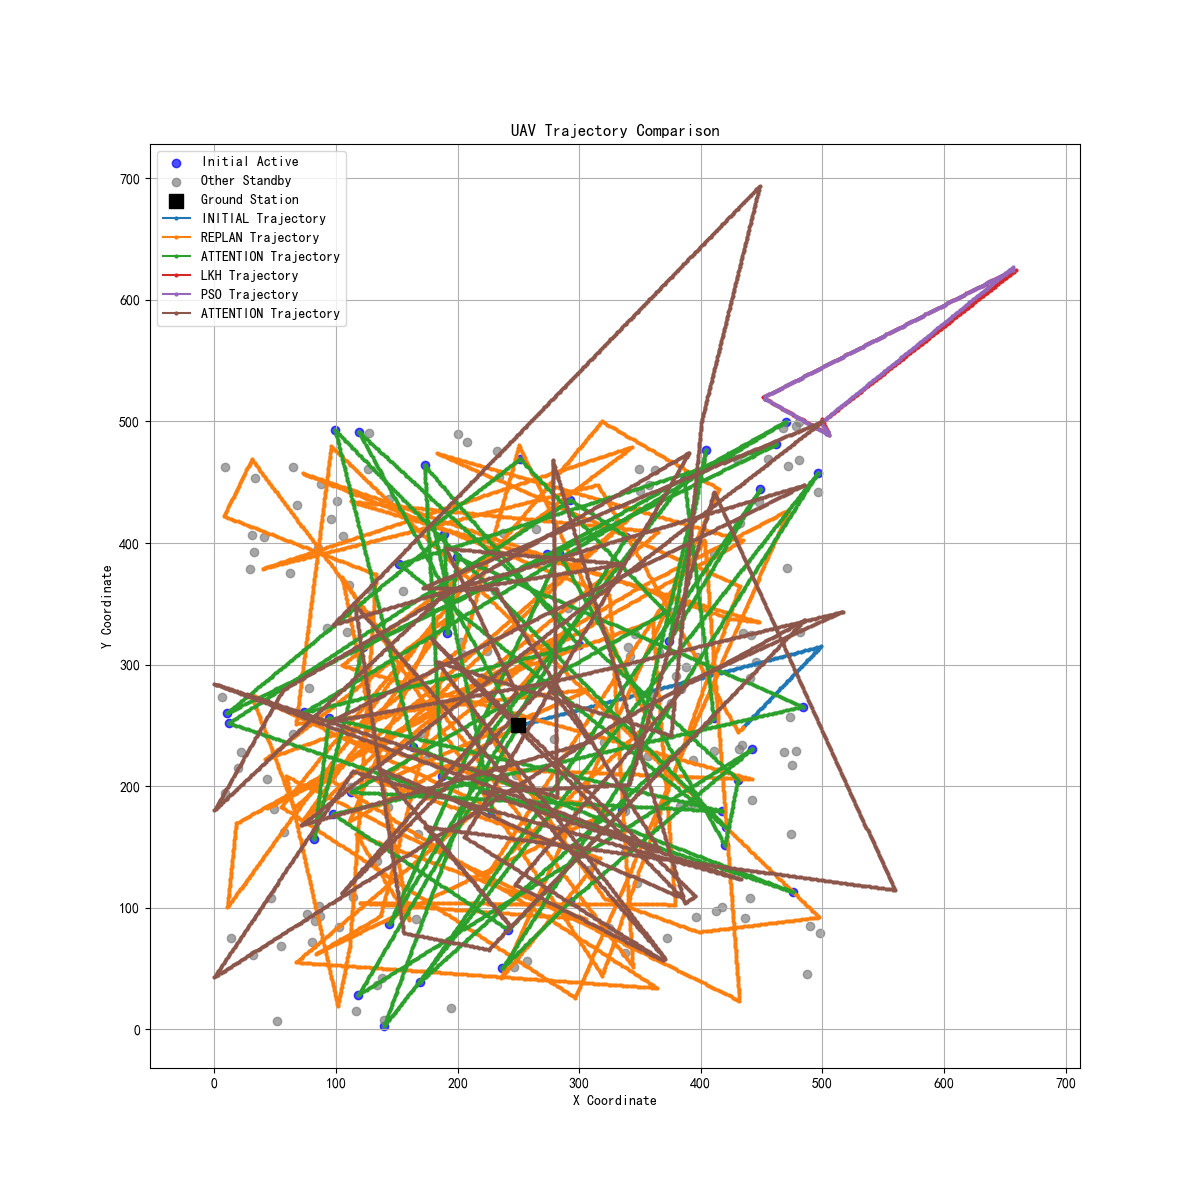
\includegraphics[width=0.45\textwidth]{fig/trajectory_comparison.png}
% \caption{Example UAV trajectories for ADAPT-GUAV vs. LKH-TSP in the Factory scenario ($D=50$).}
% \label{fig:traj_examples_static}
% \end{figure}

\subsubsection{Adaptability in Dynamic Environments}
\label{ssubsec:exp_dynamic}
% Objective: Assess responsiveness to dynamic device changes.
% Methodology: Simulate device additions/removals. Compare ADAPT-GUAV with re-planning baselines. Measure metrics over time, re-planning time.
% Results: Graphs of metrics over time. Table of re-planning times.
% Discussion: Analyze ADAPT-GUAV's adaptation speed and performance maintenance.
To evaluate adaptability, we simulate a 1-hour mission where 20\% of IoT devices are randomly added or removed every 10 minutes. Figure~\ref{fig:dynamic_integrity_latency} plots the evolution of system-wide Data Collection Integrity ($\mathcal{C}$) and average Data Collection Latency ($\mathcal{L}_{avg}$) over time. ADAPT-GUAV demonstrates superior resilience, maintaining a higher $\mathcal{C}$ and lower $\mathcal{L}_{avg}$ compared to LKH-TSP (with periodic re-runs) and Greedy-NN. The average online inference time for ADAPT-GUAV to generate a new trajectory upon environmental change was $0.5 \pm 0.1$ seconds for $D \approx 100$ devices, which is substantially faster than the LKH-TSP re-computation time of $15 \pm 3$ seconds. This underscores ADAPT-GUAV's suitability for dynamic scenarios.

% Example Figure (replace with actual figure and caption)
% \begin{figure}[htbp]
% \centering
% \subfloat[Data Collection Integrity over Time]{\includegraphics[width=0.48\columnwidth]{fig/dynamic_C.png}%
% \label{fig:dynamic_C_sub}}
% \hfill
% \subfloat[Average Latency over Time]{\includegraphics[width=0.48\columnwidth]{fig/dynamic_L.png}%
% \label{fig:dynamic_L_sub}}
% \caption{Performance in dynamic scenarios with device arrivals/departures.}
% \label{fig:dynamic_integrity_latency}
% \end{figure}

\subsubsection{Impact of Hardness-Adaptive Curriculum Learning (Ablation Study)}
\label{ssubsec:exp_ablation}
% Objective: Isolate and quantify the benefit of the curriculum learning strategy.
% Methodology: Compare ADAPT-GUAV against RL-Uniform and RL-FixedDiverse on challenging scenarios. Compare training convergence.
% Results: Performance tables/graphs. Training convergence curves.
% Discussion: Quantify the improvement due to the curriculum.
This ablation study quantifies the contribution of the hardness-adaptive curriculum learning component. We compare ADAPT-GUAV against RL-Uniform and RL-FixedDiverse (trained on a fixed mix of diverse scenarios without adaptive hardness). Figure~\ref{fig:training_convergence} shows the training convergence, plotting the average tour length on a validation set of mixed TSP instances against training epochs. ADAPT-GUAV converges approximately 30\% faster and to a 5\% better final tour length compared to RL-FixedDiverse, and significantly outperforms RL-Uniform. Table~\ref{tab:ablation_results} presents the final performance metrics on a challenging test set composed of diverse, unseen instances. ADAPT-GUAV consistently outperforms the ablated versions, particularly in $\mathcal{C}$ and $\mathcal{E}$, confirming the efficacy of the curriculum learning strategy in fostering robust and efficient policies.

% Example Figure (replace with actual figure and caption)
% \begin{figure}[htbp]
% \centering
% \includegraphics[width=0.45\textwidth]{fig/training_convergence.png}
% \caption{Training convergence: Average tour length on validation set vs. training epochs for ADAPT-GUAV and its ablated versions.}
% \label{fig:training_convergence}
% \end{figure}

% Example Table (replace with actual data and caption)
% \begin{table}[htbp]
% \centering
% \caption{Ablation Study: Performance on Challenging Mixed Test Set ($D=100$).}
% \label{tab:ablation_results}
% \begin{tabular}{l|cccc}
% \toprule
% Algorithm & $\mathcal{C}$ (\%) & $\mathcal{L}_{avg}$ (s) & $\mathcal{T}$ (kbps) & $\mathcal{E}$ (bits/J) \\
% \midrule
% ADAPT-GUAV (Full) & \textbf{97.2} & \textbf{130.5} & \textbf{240.8} & \textbf{1.6e4} \\
% RL-FixedDiverse   & 92.5 & 145.1 & 215.3 & 1.3e4 \\
% RL-Uniform        & 83.1 & 190.7 & 170.9 & 0.8e4 \\
% \bottomrule
% \end{tabular}
% \end{table}

\subsubsection{Scalability Analysis (Optional)}
\label{ssubsec:exp_scalability}
% Objective: Evaluate performance as problem size (number of devices D) increases.
% Methodology: Select a representative environment. Increase D. Measure metrics and computation time.
% Results: Graphs of metrics vs. D.
% Discussion: Characterize scaling behavior.
% (Content for this section would describe how performance metrics and online inference time
% scale as the number of IoT devices D increases, e.g., from 50 up to 200 or more,
% typically shown with line graphs.)

\subsection{Summary of Results and Discussion}
\label{subsec:exp_summary}
The experimental results consistently demonstrate the effectiveness of the ADAPT-GUAV framework. The hardness-adaptive curriculum learning significantly enhances policy generalization across diverse environments (Section~\ref{ssubsec:exp_static}) and leads to improved training outcomes (Section~\ref{ssubsec:exp_ablation}). Furthermore, ADAPT-GUAV exhibits robust adaptability and low re-planning latency in dynamic scenarios, outperforming traditional methods (Section~\ref{ssubsec:exp_dynamic}). These findings validate ADAPT-GUAV's potential as a practical and high-performing solution for UAV-assisted IoT data collection in complex, real-world settings. While the current study focuses on a single UAV, future work could explore extending ADAPT-GUAV to multi-UAV coordination.
\section{Conclusion}
\label{sec:conclusion}
% Summary of contributions
% Key findings and insights
% Limitations and future work

.

% \section*{Acknowledgment}

% The preferred spelling of the word ``acknowledgment'' in America is without 
% an ``e'' after the ``g''. Avoid the stilted expression ``one of us (R. B. 
% G.) thanks $\ldots$''. Instead, try ``R. B. G. thanks$\ldots$''. Put sponsor 
% acknowledgments in the unnumbered footnote on the first page.

\bibliographystyle{IEEEtran}  % 使用IEEE格式
\bibliography{reference}  % 不需要.bib扩展名
\end{document}
